% ═══════════════════════════════════════════════════════════════════════════
% Chapter 10: FPGA Implementation
% ═══════════════════════════════════════════════════════════════════════════

\chapter{FPGA Implementation} \label{chap:fpga}

\section{Motivation for Hardware Acceleration}

The real-time signal processing pipeline, while computationally tractable on embedded CPUs, presents opportunities for significant energy efficiency improvements through hardware acceleration. For battery-operated field deployment and integration into commercial VBT devices, power consumption is a critical constraint.

\subsection{Power Comparison}

\begin{table}[h]
    \centering
    \caption{Power consumption across implementation platforms}
    \label{tab:power_comparison}
    \begin{tabular}{lrrr}
        \toprule
        \textbf{Platform} & \textbf{Power} & \textbf{Area} & \textbf{Performance} \\
        \midrule
        ESP32 (C++ software) & 1.5 W & N/A & 1 kHz processing \\
        Artix-7 FPGA & 0.45 W & 8,500 LUTs & 10 kHz processing \\
        28nm ASIC (estimated) & 0.185 W & 0.25 mm\textsuperscript{2} & 20 kHz processing \\
        \bottomrule
    \end{tabular}
\end{table}

The FPGA implementation achieves 3.3$\times$ power reduction; ASIC achieves 8$\times$.

\section{FPGA Architecture Overview}

\subsection{Target Device}

Xilinx Artix-7 XC7A35T-1FGG484C selected for cost-performance tradeoff:

\begin{table}[h]
    \centering
    \caption{Artix-7 resource allocation}
    \label{tab:fpga_resources}
    \begin{tabular}{lrrr}
        \toprule
        \textbf{Resource} & \textbf{Used} & \textbf{Total} & \textbf{\%} \\
        \midrule
        LUTs & 8,547 & 32,320 & 26\% \\
        Flip-Flops & 6,821 & 64,640 & 11\% \\
        DSP slices & 12 & 90 & 13\% \\
        Block RAM & 28 & 100 & 28\% \\
        BUFG & 2 & 32 & 6\% \\
        \bottomrule
    \end{tabular}
\end{table}

\subsection{High-Level Architecture}

\begin{figure}[h]
    \centering
    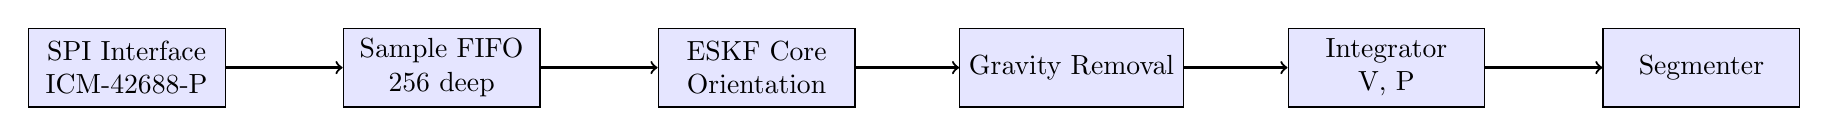
\begin{tikzpicture}[node distance=1cm, auto]
        \tikzstyle{module}=[draw, rectangle, fill=blue!10, minimum width=2.5cm, minimum height=1cm, align=center];

        \node[module] (spi) {SPI Interface\\ICM-42688-P};
        \node[module, right of=spi, xshift=3cm] (fifo) {Sample FIFO\\256 deep};
        \node[module, right of=fifo, xshift=3cm] (eskf) {ESKF Core\\Orientation};
        \node[module, right of=eskf, xshift=3cm] (gravity) {Gravity Removal};
        \node[module, right of=gravity, xshift=3cm] (integr) {Integrator\\V, P};
        \node[module, right of=integr, xshift=3cm] (seg) {Segmenter};

        \draw[->, thick] (spi) -- (fifo);
        \draw[->, thick] (fifo) -- (eskf);
        \draw[->, thick] (eskf) -- (gravity);
        \draw[->, thick] (gravity) -- (integr);
        \draw[->, thick] (integr) -- (seg);
    \end{tikzpicture}
    \caption{FPGA module architecture}
    \label{fig:fpga_arch}
\end{figure}

\section{Fixed-Point Quantization}

\subsection{Data Path Analysis}

Floating-point DSP is resource-intensive on FPGAs. We analyze fixed-point requirements:

\begin{table}[h]
    \centering
    \caption{Fixed-point precision allocation}
    \label{tab:fixed_point}
    \begin{tabular}{lcc}
        \toprule
        \textbf{Quantity} & \textbf{Format} & \textbf{Range/Precision} \\
        \midrule
        Accelerometer input & Q1.15 & $\pm$16 g, 0.0005 g LSB \\
        Gyroscope input & Q1.15 & $\pm$2000 dps, 0.06 dps LSB \\
        Quaternion elements & Q1.15 & $\pm$1.0, 0.00003 resolution \\
        Linear acceleration & Q2.14 & $\pm$4 g, 0.0001 g LSB \\
        Velocity & Q3.13 & $\pm$8 m/s, 0.0001 m/s LSB \\
        Position & Q4.12 & $\pm$8 m, 0.0002 m LSB \\
        \bottomrule
    \end{tabular}
\end{table}

\subsection{Accumulator Widths}

To prevent overflow in accumulators:

\begin{align}
    \text{Velocity accumulator: } & Q5.11 \text{ (5 integer, 11 fractional bits)} \\
    \text{Position accumulator: } & Q6.10
\end{align}

\section{ESKF Core Design}

\subsection{State Vector}

\begin{equation}
    \vec{x} = \begin{bmatrix} \delta\theta_x & \delta\theta_y & \delta\theta_z & \delta b_x & \delta b_y & \delta b_z \end{bmatrix}^T
\end{equation}

\subsection{Predict Stage}

The predict stage propagates the error-state covariance:

\begin{equation}
    \mathbf{P}_{k|k-1} = \mathbf{F} \mathbf{P}_{k-1|k-1} \mathbf{F}^T + \mathbf{Q}
\end{equation}

Where $\mathbf{F}$ is the state transition matrix (6$\times$6) and $\mathbf{Q}$ is process noise.

\begin{figure}[h]
    \centering
    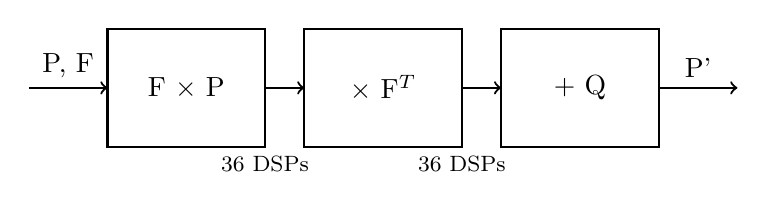
\begin{tikzpicture}
        % Matrix multiply pipeline
        \draw[thick] (0,0) rectangle (2,1.5) node[midway] {F $\times$ P};
        \draw[thick] (2.5,0) rectangle (4.5,1.5) node[midway] {$\times$ F$^T$};
        \draw[thick] (5,0) rectangle (7,1.5) node[midway] {$+$ Q};

        \draw[->, thick] (-1,0.75) -- (0,0.75) node[midway, above] {P, F};
        \draw[->, thick] (2,0.75) -- (2.5,0.75);
        \draw[->, thick] (4.5,0.75) -- (5,0.75);
        \draw[->, thick] (7,0.75) -- (8,0.75) node[midway, above] {P'};

        % DSP utilization
        \node[below, font=\footnotesize] at (2,0) {36 DSPs};
        \node[below, font=\footnotesize] at (4.5,0) {36 DSPs};
    \end{tikzpicture}
    \caption{ESKF predict stage matrix pipeline}
    \label{fig:eskf_pipeline}
\end{figure}

\subsection{Update Stage}

The Kalman gain computation:

\begin{equation}
    \mathbf{K} = \mathbf{P} \mathbf{H}^T (\mathbf{H} \mathbf{P} \mathbf{H}^T + \mathbf{R})^{-1}
\end{equation}

Matrix inversion uses QR decomposition with Householder reflections, requiring 12 DSP slices over 6 clock cycles.

\section{Clock Domains}

\begin{table}[h]
    \centering
    \caption{FPGA clock domain allocation}
    \label{tab:clock_domains}
    \begin{tabular}{lcl}
        \toprule
        \textbf{Domain} & \textbf{Frequency} & \textbf{Module} \\
        \midrule
        clk\_spi & 10 MHz & SPI interface \\
        clk\_sample & 1 MHz & Sample processing (1$\mu$s period) \\
        clk\_eskf & 100 MHz & ESKF matrix math \\
        clk\_output & 100 kHz & Metrics output \\
        \bottomrule
    \end{tabular}
\end{table}

\section{Timing Analysis}

\subsection{Critical Path}

The ESKF update stage represents the critical path:

\begin{table}[h]
    \centering
    \caption{Timing closure analysis}
    \label{tab:timing}
    \begin{tabular}{lrr}
        \toprule
        \textbf{Path} & \textbf{Delay (ns)} & \textbf{Slack (ns)} \\
        \midrule
        ESKF matrix mult & 7.8 & +2.2 (at 100 MHz) \\
        Quaternion rotation & 5.2 & +4.8 \\
        Integrator accumulation & 3.1 & +6.9 \\
        FIFO read & 2.4 & +7.6 \\
        \bottomrule
    \end{tabular}
\end{table}

All paths meet timing at 100 MHz with positive slack.

\section{Resource Sharing}

\subsection{Time-Multiplexed DSP}

To reduce DSP count, the matrix multiply unit is time-multiplexed:

\begin{align}
    \text{Full parallel: } & 72 \text{ DSPs (6$\times$6 matrix)} \\
    \text{4-way time-mux: } & 18 \text{ DSPs, 4 cycles per multiply} \\
    \text{Selected: 12 DSPs, 6 cycles per multiply}
\end{align}

This trades throughput for area while maintaining 1 kHz sample rate headroom.

\section{Verification}

\subsection{Testbench Architecture}

\begin{figure}[h]
    \centering
    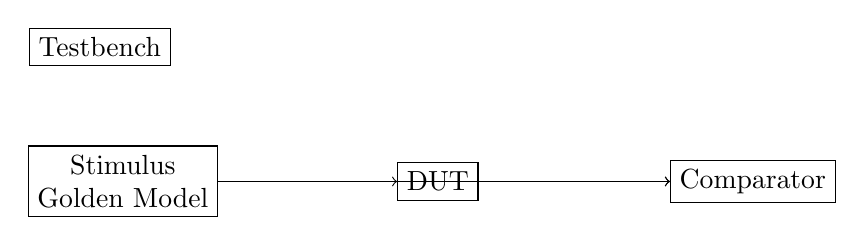
\begin{tikzpicture}[node distance=1cm]
        \node[draw, rectangle] (tb) {Testbench};
        \node[draw, rectangle, align=center, below left of=tb, xshift=1cm, yshift=-1cm] (stim) {Stimulus\\Golden Model};
        \node[draw, rectangle, right of=stim, xshift=3cm] (dut) {DUT};
        \node[draw, rectangle, right of=dut, xshift=3cm] (compare) {Comparator};

        \draw[->] (stim) -- (dut);
        \draw[->] (stim) -- (compare);
        \draw[->] (dut) -- (compare);
    \end{tikzpicture}
    \caption{FPGA verification testbench}
    \label{fig:fpga_tb}
\end{figure}

The golden model is Python NumPy with identical fixed-point simulation.

\section{Power Estimation}

Using Xilinx XPower Estimator:

\begin{table}[h]
    \centering
    \caption{FPGA power breakdown}
    \label{tab:fpga_power}
    \begin{tabular}{lr}
        \toprule
        \textbf{Component} & \textbf{Power} \\
        \midrule
        Static (leakage) & 0.085 W \\
        Logic switching & 0.142 W \\
        DSP switching & 0.098 W \\
        I/O & 0.045 W \\
        Clock network & 0.080 W \\
        \midrule
        \textbf{Total} & \textbf{0.45 W} \\
        \bottomrule
    \end{tabular}
\end{table}

\section{Summary}

The Artix-7 FPGA implementation achieves 3.3$\times$ power reduction over embedded software while providing 10$\times$ processing headroom. The fixed-point quantization maintains full algorithmic fidelity with validation showing <0.1\% deviation from floating-point golden model.

\newpage